\subsection{Sprint 5: Gestión de Vacantes}
\begin{description}
    \item \textbf{Duración}: 15 días.
    \item \textbf{Inicio del sprint }: 26 de marzo de 2022.
    \item \textbf{Cierre del sprint }: 10 de abril de 2022.
\end{description}

\subsection{Planeación}

Esta iteración tuvo como propósito implementar un mecanismo para la gestión de vacantes dentro del sistema, las actividades 
realizadas fueron:
\begin{enumerate}
    \item Se diseñó e implementó las interfaces de usuario para la gestión de vacantes según el tipo de cuenta.
    \item Se especificaron los requerimientos mediante casos de uso con sus respectivas interfaces de usuario.
    \item Se elaboró el a de casos de uso para este sprint.
    \item Se elaboró la maquina de estados de una vacante.
\end{enumerate} 

Los requerimientos funcionales de este sprint se muestran en la siguiente tabla.
\begin{requerimientos}{funcionales}
    \RFitem{RF-09}{Consultar vacantes}{El sistema debe permitir a cualquier persona consultar las vacantes que se tengan registradas siempre y cuando aun estén abiertas.}
    \RFitem{RF-10}{Publicar vacantes }{El sistema debe permitir  a los usuarios registrados publicar vacantes.}
    \RFitem{RF-11}{Editar vacantes}{El sistema debe permitir a los usuarios editar las vacantes que ellos hayan publicado.}
    \RFitem{RF-12}{Reportar vacantes}{El sistema debe permitir a los usuarios reportar vacantes publicadas si es que el usuario lo crea necesario.}
    \RFitem{RF-13}{Eliminar vacantes}{El sistema debe permitir a los usuarios eliminar las vacantes que ellos hayan publicado.}
\end{requerimientos}

Los casos de uso que se describieron en este sprint pertenecen al \textbf{Módulo Vacantes (VCT)} cuyo propósito es gestionar
todas las vacantes segun el tipo de cuenta del usuario.

En la figura \ref{dcu:MUVCT} se puede ver el diagrama de casos de uso.
\begin{itemize}
    \item Los casos de uso \IUazul{} , son aquellos que se van implementar en este sprint.
    \item Los casos de uso \IUblanco{}, se tienen planeados para sprints posteriores.
\end{itemize} 

\begin{figure}[H]
    \begin{center}
        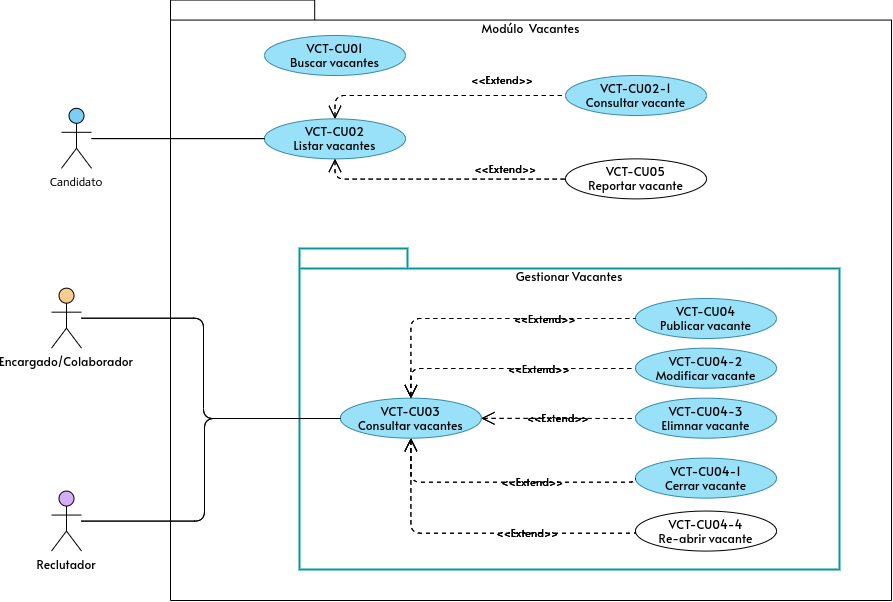
\includegraphics[width=.7\textwidth]{sprints/imagenes/MUVCT.png}
    \end{center}
    \caption{Diagrama de casos de uso del \textit{Modúlo Vacantes}.}
    \label{dcu:MUVCT}
\end{figure}

A continuación se listan los casos de uso de este sprint para el modúlo vacantes:
\begin{enumerate}
    \item \refElem{VCT-CU01}
    \item \refElem{VCT-CU02} 
    \item \refElem{VCT-CU02-1} 
    \item \refElem{VCT-CU03}
    \item \refElem{VCT-CU03-1}
    \item \refElem{VCT-CU03-2} 
    \item \refElem{VCT-CU03-3} 
\end{enumerate} 

\subsection{Ejecución}

En la elaboración del módulo de gestión de vacantes se crearon servicios para conectar el frontend con el backend y poder hacer la peticiones HTTP con el verbo GET a cada endpoint que almacena la información de cada vacante, ya sea una vacante publicada por un reclutador, una vacante a la cual postuló un candidato o para mostrar la lista de todas las vacantes y con el verbo POST a cada endpoint que reciben payloads con la información necesaria para registrar las vacantes nuevas. \\
\newline
%De lado del backend la gestión de vacantes se realiza de acuerdo con las peticiones realizadas por el frontend a través
